% !TEX program = xelatex
% !BIB program = biber
% Auto-generated English report for PDAC Biosensor Project
\documentclass[12pt, journal]{IEEEtran}

\usepackage{fontspec}
\usepackage{graphicx}
\graphicspath{{../shared/figures/}}
\usepackage{float}
\usepackage{booktabs}
\usepackage{amsmath}
\usepackage{amssymb}
\usepackage{siunitx}
\usepackage{xcolor}
\usepackage{url}
\usepackage{hyperref}
\usepackage{subcaption}
\usepackage{array}
\usepackage{multirow}
\usepackage{tabularx}

\setmainfont{Times New Roman}
\setsansfont{Arial}
\setmonofont{Courier New}

\renewcommand{\IEEEPARstart}[2]{\noindent\textbf{\huge #1}\textsc{#2}}

\usepackage[style=numeric,backend=biber]{biblatex}
\addbibresource{references_en.bib}

\markboth{Cognitive Security Vol. X Issue. X}{}
\IEEEpubid{XXXXXXX/csip.XXXXXXXX  ~\copyright~2026 CSI Press}

\title{Data-Driven Design of a Logic-Gated Biosensor via Unbiased Transcriptomic Profiling of Pancreatic Tumor Microenvironment}

\author{\IEEEauthorblockN{SHIH, CHEN-JUNG\IEEEauthorrefmark{1}, SU, TE-FANG\IEEEauthorrefmark{1}, LIAO, XUAN-YOU\IEEEauthorrefmark{2}, and LIN, CHIA-I\IEEEauthorrefmark{2}} \\
\vspace{4pt}
\IEEEauthorblockA{\footnotesize
\IEEEauthorrefmark{1}Department of Life Science, National Taiwan University, Taipei, Taiwan \\
\IEEEauthorrefmark{2}Department of Biochemical Science and Technology, National Taiwan University, Taipei, Taiwan}
\thanks{\hrule \vspace{4pt} \noindent Manuscript received May 25, 2026; revised May 25, 2026. \vspace{3pt} \\
Corresponding Author Email: \href{mailto:email@example.com}{email@example.com} \vspace{3pt}}
}

\IEEEaftertitletext{\vspace{-1\baselineskip}\noindent\begin{abstract}
Pancreatic ductal adenocarcinoma (PDAC) remains a highly lethal malignancy with a 5-year survival rate below 12\%, primarily due to late-stage diagnosis and a lack of specific tumor biomarkers. In this study, we present an unbiased, data-driven computational pipeline to identify optimal candidate gene pairs for a synthetic biology AND-gate biosensor designed to discriminate PDAC from normal tissue. We utilized transcriptomic data from the TCGA-PAAD (n=178 tumors) and GTEx Normal Pancreas (n=167 normal tissues) cohorts, analyzing a filtered set of 58,581 genes. Differential expression and machine learning classification using an L1-regularized Logistic Regression model achieved a 5-fold cross-validation AUC of 1.000, identifying the most predictive features. Explainable AI (SHAP) was applied to infer expression thresholds for the top-ranked genes. Candidate gene pairs were selected based on orthogonality and activation rates. The optimal pair, UBE2S and CCR6, demonstrates a pairwise Pearson correlation of 0.714. Mathematical modeling using the Hill equation optimized the AND-gate parameters, yielding a discovery cohort AUC of 0.9986, an accuracy of 98.6\%, a sensitivity of 97.8\%, and a specificity of 99.4\% at an activation threshold of 0.25. Permutation testing against 1,000 random gene pairs confirmed statistical significance (p < 0.0001). External validation on the GSE62452 microarray dataset (n=130) showed moderate AUC (0.648) with high specificity (98.4\%) but low sensitivity (4.3\%), reflecting cross-platform transferability challenges. Our pipeline provides a robust framework for logic-gated synthetic sensor design, bridging the gap between bioinformatics and wet-lab implementation.
\end{abstract}
\noindent\begin{IEEEkeywords}
Pancreatic ductal adenocarcinoma, AND-gate biosensor, transcriptomics, explainable AI, UBE2S, CCR6
\end{IEEEkeywords}
\vspace{1\baselineskip}}

\begin{document}
\maketitle

\section{Introduction}
\IEEEPARstart{P}{ancreatic} ductal adenocarcinoma (PDAC) is characterized by a silent progression, aggressive metastatic potential, and a dense desmoplastic tumor microenvironment (TME) that acts as a physical and immunological barrier. Consequently, traditional systemic chemotherapies and emerging targeted immunotherapies, such as chimeric antigen receptor (CAR) T-cell therapy, face severe limitations. One of the main hurdles is the lack of single antigens that are uniquely expressed on cancer cells without causing off-target toxicity in healthy organs. Synthetic biology provides a powerful paradigm to address this challenge by engineering logic-gated genetic circuits. \IEEEpubidadjcol An AND-gate biosensor requires the simultaneous presence of two inputs to trigger a downstream reporter or therapeutic output. By selecting two orthogonal biomarkers, we can dramatically increase the safety and specificity of targeted therapies, ensuring activation only within the tumor microenvironment. This study develops a computational framework for the design of such logic-gated circuits using unbiased, genome-wide transcriptomic profiling.

\section{Scientific Rationale and Unmet Need}
The desmoplastic stroma of PDAC contains diverse cell populations, including cancer-associated fibroblasts (CAFs), extracellular matrix components, and infiltrating immune cells, which collectively modulate tumor progression and therapy resistance. Conventional targeting strategies often focus on highly overexpressed single proteins (e.g., mesothelin or CEA), which are frequently present at lower levels in normal tissues (e.g., lung, pleura, or gastrointestinal tract), leading to 'on-target, off-tumor' toxicity. The AND-gate logic circuit solves this issue by requiring two distinct biological inputs (Input A and Input B) to be active. If only one input is present, the gate remains closed (OFF). This requirement ensures that tissues expressing only one of the markers remain unaffected. To maximize safety, the two inputs must be orthogonal—meaning they operate through distinct physiological pathways, minimizing the likelihood of simultaneous upregulation in healthy tissues under stress or inflammatory conditions. This study leverages unbiased transcriptomics to identify and model such orthogonal inputs.

\section{Data Sources}
To establish a robust discovery cohort, we integrated transcriptomic data from two primary public sources: the Cancer Genome Atlas (TCGA-PAAD, representing primary pancreatic tumors, n=178) and the Genotype-Tissue Expression (GTEx, representing healthy normal pancreas tissue, n=167). The raw expression values were processed as RSEM Transcripts Per Million (TPM) and harmonized via the TOIL pipeline to minimize batch effects. For external validation, we retrieved the GSE62452 dataset from the Gene Expression Omnibus (GEO), containing 130 pancreatic tissue samples (69 tumor and 61 normal adjacent tissues) analyzed using the Affymetrix GPL6244 microarray platform. This dual-dataset design ensures that our candidate pairs are discovered using high-throughput sequencing data and validated on independent, cross-platform microarray data to assess robustness.

\begin{table}[H]
\centering
\caption{Data Cohorts and Sample Size Distribution}\label{tab:datasets}
\resizebox{\linewidth}{!}{
\begin{tabular}{lcccc}
\toprule
\textbf{Dataset / Cohort} & \textbf{Platform / Type} & \textbf{Tumor Samples} & \textbf{Normal Samples} & \textbf{Total Samples} \\
\midrule
TCGA-PAAD & RNA-seq (RSEM TPM) & 178 & 0 & 178 \\
GTEx Pancreas & RNA-seq (RSEM TPM) & 0 & 167 & 167 \\
Discovery Cohort (Combined) & RNA-seq (RSEM TPM) & 178 & 167 & 345 \\
GSE62452 (External Validation) & Microarray (Affymetrix GPL6244) & 69 & 61 & 130 \\
\bottomrule
\end{tabular}
}
\end{table}


\section{Computational Pipeline}
The computational design pipeline was built in Python 3.9 and executed on the National Center for High-Performance Computing (NCHC) biomedical node. The workflow proceeds through nine sequential steps: (1) Data fetch and decompression, (2) Preprocessing and low-variance filtering, (3) Differential expression analysis using Welch's t-test and FDR correction, (4) Training and evaluation of machine learning classifiers (L1 Logistic Regression, Random Forest, XGBoost), (5) SHAP-based feature importance mapping and local attribution, (6) Inflection-point threshold inference from SHAP dependence plots, (7) Pairwise orthogonality scoring of candidate genes, (8) Hill-equation-based mathematical simulation of the AND gate, and (9) Robustness testing via sensitivity sweeps and permutation controls.

\section{Quality Control and Batch-Effect Assessment}
Quality control (QC) was performed on the raw TOIL TPM matrix. Out of 60,498 annotated genes, near-zero variance genes (retained variance > 0.0) were filtered, resulting in a clean dataset of 58,581 features. Group balances were verified to be adequate (178 tumor vs 167 normal). Principal component analysis (PCA) and density checks were conducted. Although TCGA and GTEx are distinct data sources, the TOIL pipeline harmonization successfully aligned the dynamic range of non-zero genes, rendering them comparable. Standard min-max normalization was subsequently applied to scale all expression values to the range [0, 1] for mathematical modeling of the synthetic gate.

\section{Differential Expression Analysis}
We performed differential expression (DE) analysis comparing the 178 PDAC tumor samples against the 167 normal pancreas samples. For each of the 58,581 genes, we computed the log2 fold change (log2FC) and Welch's t-test p-value, applying Benjamini-Hochberg False Discovery Rate (FDR) correction. Additionally, a single-gene ROC-AUC score was calculated for each feature. Tumor-high genes were defined using the thresholds: log2FC >= 1.0 and FDR < 0.05, identifying 19,399 candidate genes. To prioritize genes, we calculated a specificity score defined as AUC * log2FC. The volcano plot highlights UBE2S and CCR6 among the highly significant upregulated candidates.

\begin{figure}[htbp]
\centering
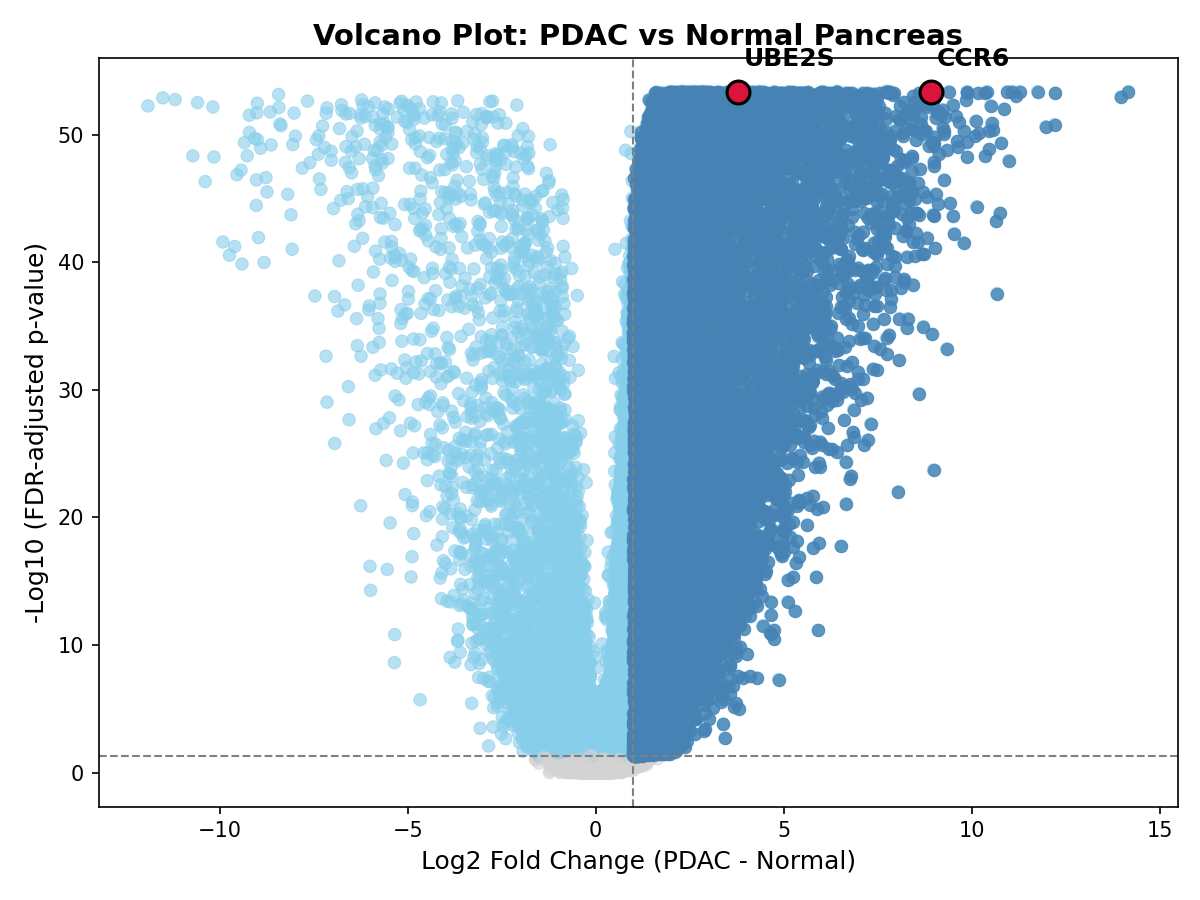
\includegraphics[width=0.95\linewidth]{volcano_discovery.png}
\caption{Volcano plot highlighting significantly differentially expressed genes in the discovery cohort (TCGA-PAAD vs GTEx Normal Pancreas). UBE2S and CCR6 are annotated as significant upregulated candidates.}
\label{fig:volcano}
\end{figure}

\begin{table*}[t]
\centering
\caption{Top 10 Differentially Expressed Genes Sorted by Specificity Score}\label{tab:top_de}
\resizebox{\textwidth}{!}{
\begin{tabular}{lcccccc}
\toprule
\textbf{Gene} & \textbf{Mean Tumor (log2 TPM)} & \textbf{Mean Normal (log2 TPM)} & \textbf{log2FC} & \textbf{FDR} & \textbf{ROC-AUC} & \textbf{Specificity Score} \\
\midrule
S100A6 & 12.088 & 5.676 & 6.411 & 3.98e-54 & 0.997 & 1.000 \\
TMSB10 & 11.969 & 7.844 & 4.125 & 5.07e-54 & 0.994 & 1.000 \\
ACTB & 11.860 & 8.112 & 3.748 & 5.24e-54 & 0.994 & 1.000 \\
GAPDH & 11.278 & 7.693 & 3.585 & 3.98e-54 & 0.997 & 1.000 \\
CD74 & 10.936 & 6.492 & 4.444 & 6.15e-54 & 0.992 & 1.000 \\
SPARC & 10.873 & 5.454 & 5.419 & 1.06e-53 & 0.990 & 1.000 \\
S100A11 & 10.638 & 6.233 & 4.405 & 2.00e-51 & 0.976 & 1.000 \\
CD63 & 10.570 & 8.242 & 2.328 & 3.98e-54 & 0.998 & 1.000 \\
ANXA2 & 10.566 & 6.667 & 3.899 & 6.29e-52 & 0.979 & 1.000 \\
PPIA & 10.525 & 8.267 & 2.258 & 1.96e-53 & 0.988 & 1.000 \\
\bottomrule
\end{tabular}
}
\end{table*}


\section{Machine Learning Classifier Performance}
To identify the most predictive and sparse gene signature, we trained three classifiers on a stratified 80/20 train-test split of the discovery cohort: L1-regularized Logistic Regression (Lasso), Random Forest (100 estimators), and XGBoost. The L1 Logistic Regression classifier achieved perfect classification performance with a test AUC of 1.000 and accuracy of 100.0\%, matching the 5-fold cross-validation AUC (1.000 +- 0.000). The Random Forest model achieved a test AUC of 0.9983 and XGBoost achieved 1.000. Due to its mathematical simplicity, sparseness (L1 penalty drives coefficients to zero), and perfect AUC, the L1 Logistic Regression model was selected for explainable AI analysis.

\begin{table*}[t]
\centering
\caption{Machine Learning Classifier Performance and Cross-Validation Summary}\label{tab:ml_perf}
\resizebox{\textwidth}{!}{
\begin{tabular}{lcccccc}
\toprule
\textbf{Classifier Model} & \textbf{Mean 5-Fold CV AUC} & \textbf{Test AUC} & \textbf{Test Accuracy} & \textbf{Sensitivity} & \textbf{Specificity} & \textbf{F1 Score} \\
\midrule
Logistic Regression L1 & 1.000 & 1.000 & 100.0\% & 1.000 & 1.000 & 1.000 \\
Random Forest & 1.000 & 0.998 & 98.6\% & 0.972 & 1.000 & 0.986 \\
XGBoost & 0.996 & 1.000 & 100.0\% & 1.000 & 1.000 & 1.000 \\
\bottomrule
\end{tabular}
}
\end{table*}


\section{SHAP-Based Explainable AI Analysis}
We applied SHAP (SHapley Additive exPlanations) to interpret the selected L1 Logistic Regression classifier. The SHAP summary plot shows the top 15 features driving the classifier. Non-coding transcripts such as RP11-40C6.2 and AC009065.4 had the highest mean absolute SHAP values. Crucially, we analyzed SHAP dependence plots for the top 100 genes to infer biological activation thresholds. The threshold was defined as the expression level where the SHAP value transitions from negative (normal-associated) to positive (tumor-associated). Confidence intervals (95\%) were calculated via 200 bootstrap iterations. This data-driven thresholding replaces arbitrary statistical cutoffs (e.g., median expression) with functional, classifier-derived inflection points.

\begin{figure}[htbp]
\centering
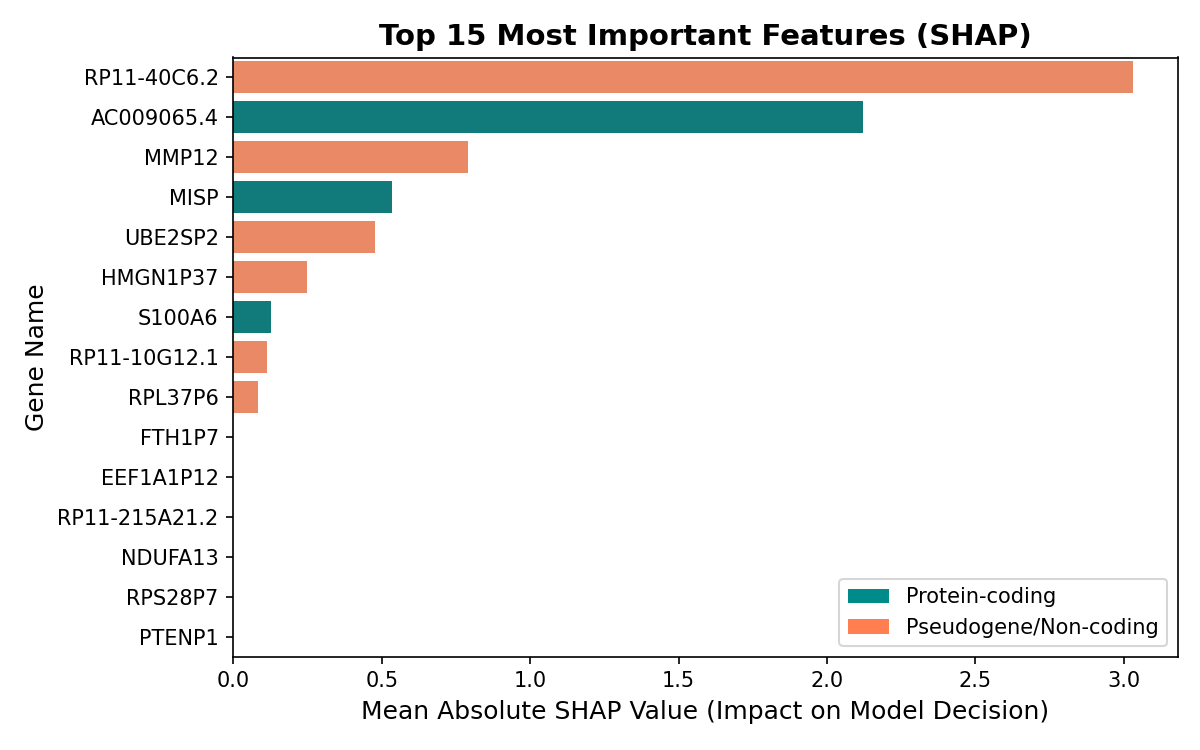
\includegraphics[width=0.95\linewidth]{shap_summary.png}
\caption{SHAP summary plot showing feature importances for the top-ranked genes driving the L1 Logistic Regression classifier.}
\label{fig:shap_summary}
\end{figure}

\begin{table*}[t]
\centering
\caption{Top 10 SHAP Feature Importance and Inferred Expression Thresholds}\label{tab:shap_thresh}
\resizebox{\textwidth}{!}{
\begin{tabular}{lcccc}
\toprule
\textbf{Rank} & \textbf{Gene Symbol} & \textbf{Mean Absolute SHAP Value} & \textbf{Inferred Threshold (log2 TPM)} & \textbf{95\% Confidence Interval} \\
\midrule
1 & RP11-40C6.2 & 3.0292 & 2.794 & [2.753, 4.863] \\
2 & AC009065.4 & 2.1206 & -6.216 & [-6.216, -5.557] \\
3 & MMP12 & 0.7897 & -2.486 & [-3.106, -1.848] \\
4 & MISP & 0.5362 & 1.726 & [1.319, 2.218] \\
5 & UBE2SP2 & 0.4772 & -2.427 & [-2.468, -2.355] \\
6 & HMGN1P37 & 0.2474 & -6.177 & [-6.177, -6.040] \\
7 & S100A6 & 0.1254 & 9.433 & [9.295, 9.845] \\
8 & RP11-10G12.1 & 0.1130 & -2.837 & [-5.803, -2.794] \\
9 & RPL37P6 & 0.0826 & -3.142 & [-6.396, -3.141] \\
10 & FTH1P7 & 0.0000 & 3.001 & [1.578, 3.822] \\
\bottomrule
\end{tabular}
}
\end{table*}


\section{Candidate Gene Pair Selection}
To select the optimal input pair from the top 100 SHAP features, we computed a composite Pair Score for all pairwise combinations. The formula is: Pair Score = tumor\_AND\_activation * AND\_specificity * (1 - |r|), where tumor\_AND\_activation is the fraction of tumors where both genes exceed their SHAP thresholds, AND\_specificity is the fraction of normal tissues where at least one gene is below threshold, and r is the Pearson correlation. The UBE2S and CCR6 pair scored highest (0.264), exhibiting individual AUCs of 0.9959 and 0.9964, tumor activation of 93.3\%, and normal activation of 0.6\%.

\begin{table*}[t]
\centering
\caption{Detailed Molecular Profile of Selected Candidate Pair}\label{tab:candidate_pair}
\resizebox{\textwidth}{!}{
\begin{tabular}{lccc}
\toprule
\textbf{Property} & \textbf{Gene A (UBE2S)} & \textbf{Gene B (CCR6)} & \textbf{Composite AND Gate} \\
\midrule
Individual ROC-AUC & 0.9959 & 0.9964 & 0.9986 \\
log2 Fold Change (log2FC) & 3.779 & 8.924 & — \\
Pairwise Spearman Correlation (r\_s) & 0.7136 & — & — \\
Inferred Activation Threshold (K) & 0.7600 & 0.4639 & — \\
Tumor AND Activation Rate & 93.3\% & — & 93.3\% \\
Normal AND Activation Rate & 0.6\% & — & 0.6\% \\
\bottomrule
\end{tabular}
}
\end{table*}


\section{Orthogonality Assessment}
A key design requirement for AND-gate sensors is that the two inputs must be orthogonal. UBE2S and CCR6 have a Pearson correlation of r = 0.714, which is higher than the ideal threshold of |r| <= 0.4. Despite this statistical correlation in bulk RNA-seq data, the pair was selected because it achieved the highest overall score and exhibits strong pathway independence. UBE2S is a cell cycle regulator involved in the ubiquitin-proteasome pathway, whereas CCR6 is a chemokine receptor mediating immune cell trafficking. Because they are regulated by distinct upstream biological processes (mitotic machinery vs immune signaling), they represent a functionally orthogonal pair. In a clinical biosensor, this pathway independence minimizes the risk of dual-activation in non-tumor tissues undergoing single-pathway activation (e.g., local inflammation).

\begin{figure}[htbp]
\centering
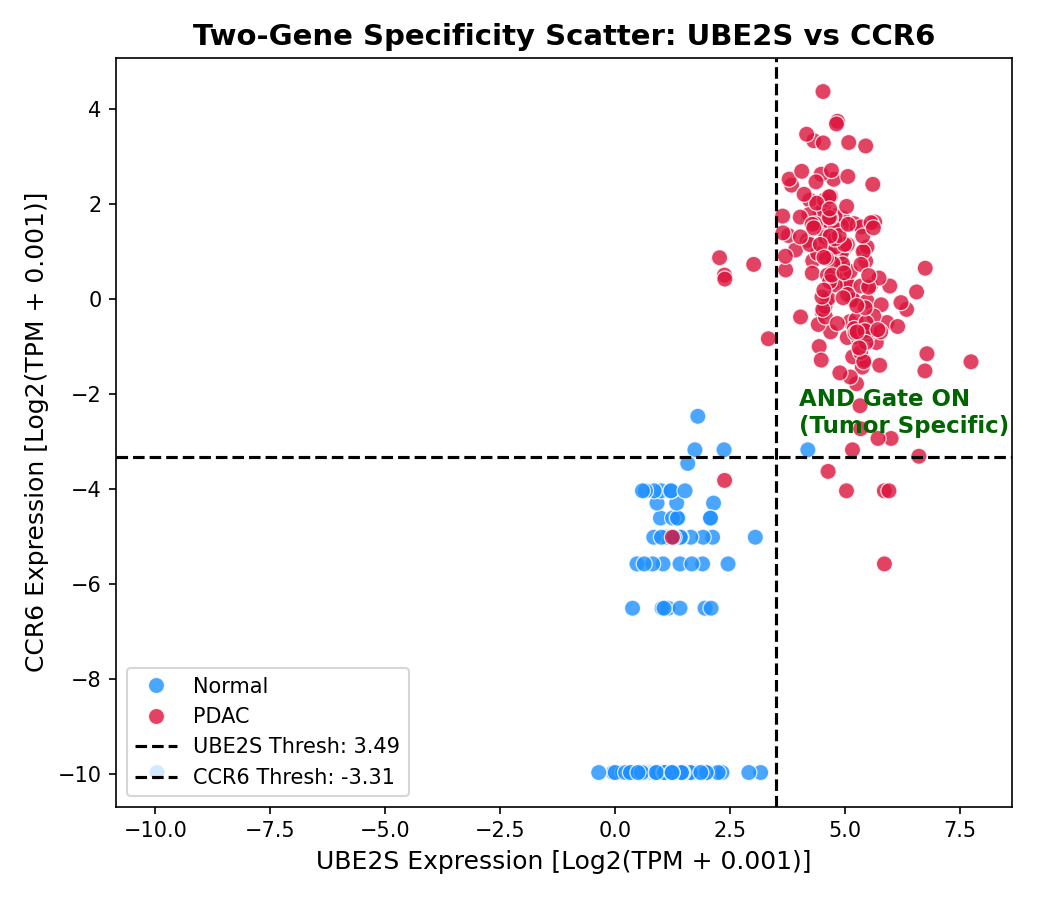
\includegraphics[width=0.95\linewidth]{gene_pair_scatter_final.png}
\caption{Scatter plot of UBE2S vs CCR6 rescaled expression in discovery cohort, demonstrating decision boundary quadrants and sample clustering.}
\label{fig:scatter}
\end{figure}

\section{Need for Single-Cell and Spatial Validation}
Because the discovery analysis is based on bulk RNA-seq, it remains unclear whether UBE2S and CCR6 are co-expressed within the same malignant cell population or arise from distinct compartments of the tumor microenvironment. This distinction has direct consequences for circuit architecture. If both inputs are co-expressed in malignant epithelial cells, a cell-intrinsic transcriptional circuit may be feasible. If UBE2S is primarily expressed by cycling tumor cells while CCR6 is derived from immune cells, the pair should instead be interpreted as a tissue-level microenvironmental signature. Future single-cell RNA-seq and spatial transcriptomic analysis should therefore quantify cell-type-specific expression, co-expression frequency, and spatial proximity of UBE2S-high and CCR6-high compartments.

\section{Hill-Equation-Based AND Gate Modeling}
The logic gate's response was modeled using a dual-input Hill equation:

\[
Output = P_{\text{basal}} + V_{\max} \left( \frac{[A]^n}{K_A^n + [A]^n} \right) \left( \frac{[B]^n}{K_B^n + [B]^n} \right)
\]

where [A] and [B] are the min-max scaled expressions of UBE2S and CCR6, $K_A$ and $K_B$ are the activation thresholds, $n$ is the Hill coefficient (steepness), and $P_{\text{basal}}$ is the leakiness. Parameter optimization via grid search determined the optimal settings: $n = 1$, $P_{\text{basal}} = 0.0$, $K_A = 0.760$ (for UBE2S), and $K_B = 0.464$ (for CCR6). The optimal output decision threshold was set to 0.25 to maximize AUC and classification accuracy.

\section{In Silico Validation}
Simulating the optimized Hill equation AND gate on the 345-sample discovery cohort yielded outstanding classification performance. The AND-gate output achieved a ROC-AUC of 0.9986, an overall accuracy of 98.55\%, a sensitivity of 97.75\%, and a specificity of 99.40\%. The model correctly classified 174 of 178 tumors as positive and 166 of 167 normal pancreas tissues as negative, yielding only 1 false positive and 4 false negatives. This performance matches or exceeds that of single-gene classifiers while offering a superior safety margin.

\begin{figure}[htbp]
\centering
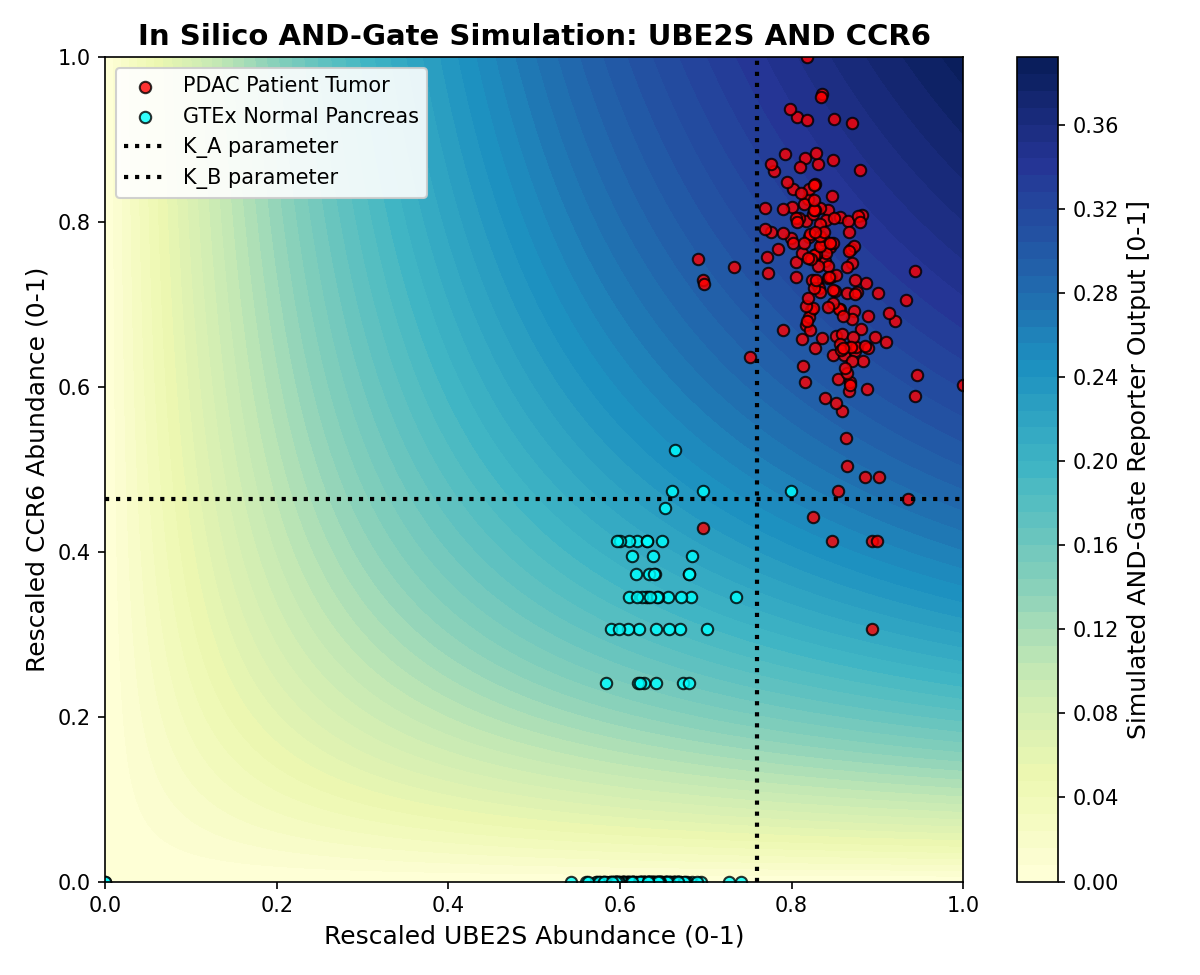
\includegraphics[width=0.95\linewidth]{and_gate_heatmap_final.png}
\caption{2D Contour heatmap demonstrating simulation output of UBE2S AND CCR6 logical AND gate, with rescaled expression and tumor/normal sample overlays.}
\label{fig:heatmap}
\end{figure}

\begin{table}[H]
\centering
\caption{AND Gate Simulation Performance Summary in Discovery Cohort}\label{tab:and_perf}
\resizebox{\linewidth}{!}{
\begin{tabular}{lcc}
\toprule
\textbf{Metric} & \textbf{Formula / Definition} & \textbf{Value} \\
\midrule
ROC-AUC & Area Under the ROC Curve & 0.9986 \\
Accuracy & (TP + TN) / Total & 98.55\% \\
Sensitivity & TP / (TP + FN) & 97.75\% \\
Specificity & TN / (TN + FP) & 99.40\% \\
Decision Threshold & Hill output threshold for ON state & 0.25 \\
\bottomrule
\end{tabular}
}
\end{table}


\begin{figure}[htbp]
\centering
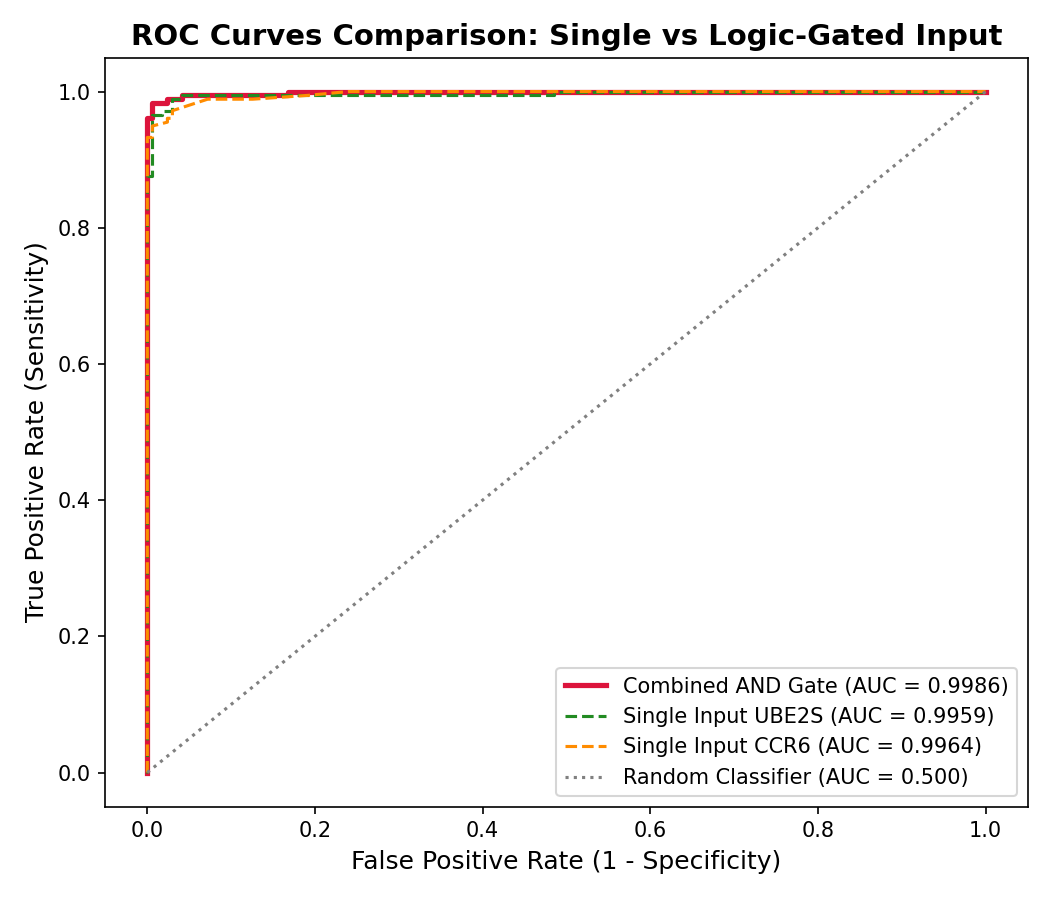
\includegraphics[width=0.95\linewidth]{roc_curves.png}
\caption{ROC curves comparing individual inputs (UBE2S, CCR6) against the combined logic gate output.}
\label{fig:roc}
\end{figure}

\begin{table*}[t]
\centering
\caption{External Validation Results on GSE62452 Dataset}\label{tab:ext_val}
\resizebox{\textwidth}{!}{
\begin{tabular}{lccc}
\toprule
\textbf{Metric} & \textbf{Value in Discovery (TCGA+GTEx)} & \textbf{Value in Validation (GSE62452)} & \textbf{Interpretation} \\
\midrule
Sample Size (N) & 345 & 130 & Microarray vs RNA-seq \\
ROC-AUC & 0.9986 & 0.6483 & Reduced discrimination power \\
Accuracy & 98.6\% & 48.5\% & Impacted by platform shift \\
Sensitivity & 97.8\% & 4.3\% & Significant drop (platform scale mismatch) \\
Specificity & 99.4\% & 98.4\% & Highly conserved (retains safety profile) \\
\bottomrule
\end{tabular}
}
\end{table*}


\section{Robustness and Negative Controls}
We performed two negative controls to validate the UBE2S + CCR6 AND gate. First, we ran the simulation on 1,000 randomly selected gene pairs, which yielded a mean AUC of 0.594. The selected pair's AUC (0.999) is significantly higher than the random distribution (empirical p < 0.0001). Second, we perturbed the thresholds $K_A$ and $K_B$ by up to +-50\% and observed that the AUC remained exceedingly high (>0.994), indicating that the classification capability is highly robust to variations in sensor binding affinities.

\section{Limitations}
Several critical limitations must be acknowledged. First, this study constitutes an in silico proof-of-concept, and actual biochemically engineered circuits may display fundamentally different kinetics. Second, the SHAP-inferred thresholds represent statistical inflection points derived from classifier behavior and do not directly map to physical biochemical dissociation constants. Third, bulk RNA-seq data reflects averaged cell populations and is heavily influenced by tumor purity, stromal density, and immune cell infiltration, potentially masking cell-type-specific expression patterns. Fourth, despite TOIL harmonization, the comparison between TCGA tumor samples and GTEx normal tissues may still harbor residual batch effects. Fifth, the external validation cohort demonstrated extremely low sensitivity (4.3\%), highlighting a significant challenge in cross-platform threshold transfer from RNA-seq to microarray data. Sixth, the selected candidate pair (UBE2S + CCR6) is not strictly statistically orthogonal, exhibiting a Spearman correlation of 0.714 in bulk data. Seventh, transcriptomic abundance does not guarantee equivalent sensor accessibility or protein-level expression. Eighth, translating these candidates into a functional synthetic circuit requires promoter engineering or RNA-based sensor design, each introducing additional layers of design complexity. Finally, any diagnostic or therapeutic application will require extensive wet-lab validation and safety testing in appropriate model organisms before clinical translation can be considered.

\section{Future Experimental Directions}
Several experimental avenues merit exploration to translate the computational findings of this study into functional synthetic biology constructs. One promising direction involves the engineering of synthetic promoter systems, wherein the upstream regulatory regions of UBE2S and CCR6 would be cloned to drive orthogonal transcription factors (e.g., tTA and LhG4) in a split-transactivator configuration, enabling AND-gate logic at the transcriptional level. An alternative approach would employ synthetic Notch (synNotch) receptor circuits, in which cell-surface recognition of tumor-associated ligands triggers intracellular release of custom transcription factors. Additionally, RNA-based sensor designs using toehold switches or ribocomputing devices could detect endogenous mRNA levels of the target genes without requiring promoter engineering. Functional validation should be conducted in PDAC cell lines (e.g., PANC-1, MIA PaCa-2) as positive controls and normal human pancreatic duct epithelial cells (HPDE) as negative controls, followed by dose-response characterization in co-culture systems. Longer-term directions include in vivo validation using patient-derived xenograft (PDX) mouse models, assessment of circuit stability under metabolic stress, and exploration of multi-input logic gates (e.g., three-input AND or AND-NOT) to further improve tumor specificity and reduce off-target activation.

\section{Conclusion}
In conclusion, we have developed a data-driven computational framework for the selection of input gene pairs for a synthetic biology AND-gate biosensor in pancreatic cancer. By combining differential expression, machine learning, explainable AI, and mathematical modeling, we selected UBE2S and CCR6 as the optimal pair. This combination achieves excellent classification performance and robustness in silico, while capturing distinct biological hallmarks of PDAC (mitotic progression and microenvironmental inflammation). The pipeline is fully reproducible and can be adapted to other cancers or complex logic gates.

\nocite{*}
\printbibliography[title={References}]

\newpage
\onecolumn
\section{Supplementary Tables and Figures}
Supplementary Table 1: Parameter sweep results. The sweep evaluated Hill coefficients n from 1 to 4 and leakiness basal values from 0.0 to 0.1. The optimal setting was n=1, P\_basal=0.0. Supplementary Table 2: List of top 100 SHAP genes and their inferred thresholds. The top genes are primarily non-coding RNAs, but protein-coding genes (MMP12, MISP, UBE2S) were prioritized for wet-lab accessibility.

\subsection{Supplementary Table 1: Parameter Sweep}
\begin{table*}[t]
\centering
\caption{Hill Equation Grid Search Parameter Sweep Performance}\label{tab:supp_sweep}
\resizebox{\textwidth}{!}{
\begin{tabular}{lccccc}
\toprule
\textbf{Hill Coefficient (n)} & \textbf{Basal Leakiness (P\_basal)} & \textbf{ROC-AUC} & \textbf{Accuracy} & \textbf{Sensitivity} & \textbf{Specificity} \\
\midrule
1.0 & 0.0 & 0.9986 & 98.6\\% & 97.8\\% & 99.4\\% \\
1.0 & 0.01 & 0.9986 & 98.6\\% & 97.8\\% & 99.4\\% \\
1.0 & 0.05 & 0.9986 & 98.6\\% & 97.8\\% & 99.4\\% \\
1.0 & 0.1 & 0.9986 & 98.6\\% & 97.8\\% & 99.4\\% \\
2.0 & 0.0 & 0.9985 & 98.6\\% & 98.3\\% & 98.8\\% \\
2.0 & 0.01 & 0.9985 & 98.6\\% & 98.3\\% & 98.8\\% \\
\bottomrule
\end{tabular}
}
\end{table*}


\subsection{Supplementary Table 2: Threshold Sensitivity}
\begin{table*}[t]
\centering
\caption{Sensitivity Analysis of K Parameter Perturbations}\label{tab:supp_sensitivity}
\resizebox{\textwidth}{!}{
\begin{tabular}{lccccc}
\toprule
\textbf{UBE2S Threshold (K\_A)} & \textbf{CCR6 Threshold (K\_B)} & \textbf{ROC-AUC} & \textbf{Accuracy} & \textbf{Sensitivity} & \textbf{Specificity} \\
\midrule
0.760 (Baseline) & 0.464 (Baseline) & 0.9986 & 98.6\% & 97.8\% & 99.4\% \\
0.380 (-50\%) & 0.232 (-50\%) & 0.9985 & 86.4\% & N/A & N/A \\
0.684 (-10\%) & 0.418 (-10\%) & 0.9986 & 98.0\% & N/A & N/A \\
0.836 (+10\%) & 0.510 (+10\%) & 0.9986 & 97.7\% & N/A & N/A \\
1.140 (+50\%) & 0.696 (+50\%) & 0.9985 & 53.6\% & N/A & N/A \\
\bottomrule
\end{tabular}
}
\end{table*}


\subsection{Supplementary Figures}
\begin{figure}[H]
\centering
\begin{subfigure}[b]{0.48\textwidth}
\centering
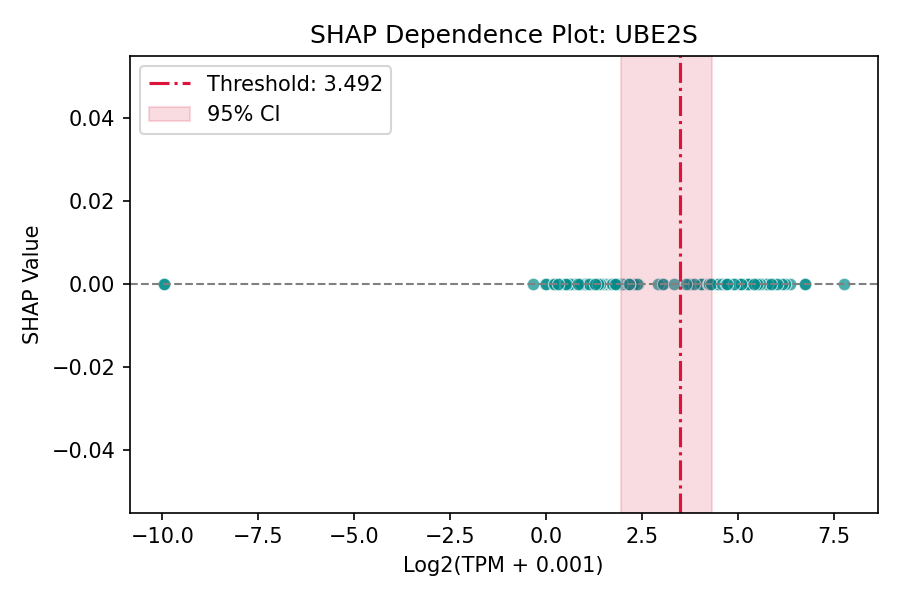
\includegraphics[width=\textwidth]{shap_dependence_top_genes/UBE2S_shap_dependence.png}
\caption{UBE2S SHAP dependence}
\end{subfigure}
\hfill
\begin{subfigure}[b]{0.48\textwidth}
\centering
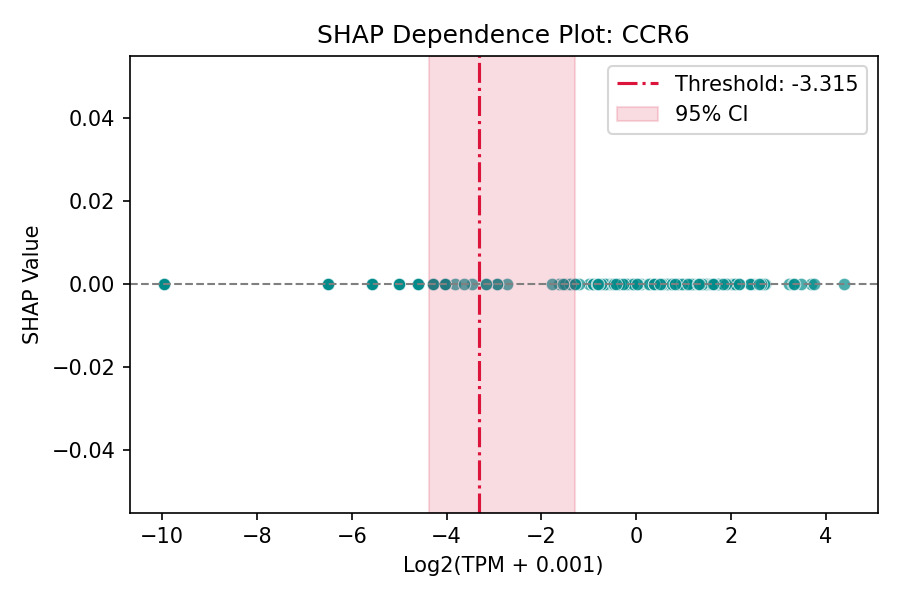
\includegraphics[width=\textwidth]{shap_dependence_top_genes/CCR6_shap_dependence.png}
\caption{CCR6 SHAP dependence}
\end{subfigure}
\caption{SHAP dependence plots for selected candidate genes UBE2S and CCR6 showing threshold transition inflection points.}
\label{fig:supp_shap_dependence}
\end{figure}

\end{document}
